\documentclass[a4paper, 11pt]{article}
\usepackage{comment} % enables the use of multi-line comments (\ifx \fi) 
\usepackage{lipsum} %This package just generates Lorem Ipsum filler text. 
\usepackage{fullpage} % changes the margin
\usepackage{bm}
\usepackage{graphicx}
\usepackage{blindtext}
\usepackage{listings}
\usepackage{amsmath}
\usepackage{setspace}
\usepackage[colorlinks=true, linkcolor=blue,urlcolor  = blue]{hyperref}
\linespread{1.5}
\begin{document}
%Header-Make sure you update this information!!!!
\noindent
Cmpsci585\\
Progress Reportl\\
Patrick Carron \\
Raymond Zhu\\
11/11/2016 \\
\begin{center}

\textbf{Predicting Political Party Affiliation from Speech}
\end{center}
\section{Introduction}
We are predicting a speaker's political party affiliation based on the language used in their congressional speeches. Based on our project proposal feedback we decided against scraping presidential campaign speeches and focus on the data which we have already procured. We are using the \href{http://www.cs.cornell.edu/home/llee/data/convote.html}{Congressional speeches dataset} created by Lillian Lee at Cornell. The dataset has been preprocessed somewhat and split into train, dev, and test sets.  We have preformed some exploratory data analysis to ensure high data quality and understand some idiosyncrasies of this data asset. We used Scikit Learn to create a data analysis pipeline so ensure that we have consistency in how the data is being processed while we search for optimal hyper parameters with different classification methods. So far we have implemented a baseline Naive Bayes classifier and a Support Vector Machine classifier with default parameters and found that our accuracies are similar to those described in our literature review.

\section{Dataset}
We began our analysis with an inspection of the congressional speech dataset. There appears to have been some preprocessing done to the speeches to support parsing. The tokens have been forced to lower case and spaces exist around select punctuation marks like periods and question marks so they are counted as separate tokens while reading in the file. The corpus contains some terms like `mr.' , however, that include punctuation as part of the token. Congressional names have been stripped from the text and replaced with unique identifiers.  The filenames contain information about the speaker including their political party affiliation. We wrote code to parse the file name and record party affiliation while reading in each individual document so we could create labels for our documents. One interesting property of this dataset is that documents are also organized around proposed legislation with some speakers voting for and against each bill in the corpus. This seems to stop idiosyncratic terms associated with specific policies from being dominated by one political party. The training set is comprised of 5,660 documents containing 1,359,493 total tokens with a vocabulary size of 23,417 terms. The test set is comprised of 1,759 documents. We used the same methodology to read in both sets of documents and record their labels.\\

\noindent
After reviewing the data set and reading documentation on several natural language processing libraries, we decided to use Scikit Learn.  Specifically, Scikit Learn offers the ability to create data pipelines and transform our feature vectors easily and consistently while preforming a set of experiments. Within our pipeline, we are using Scikit Learn's feature extraction library to create word count vectors and train our classifiers. This package will allow us to test the impact of TF-IDF weighting on our classification accuracy, along with searching over different length language models to determine which is most predictive. We used the CountVectorizer function to create a sparse matrix representation of the terms in the corpus. We reviewed basic word count and vocabulary statistics to insure that the CountVectorizor function was performing as expected. The ten most commonly used terms and frequencies matched our expectations because the list is largely comprised of determiners, conjunctions, and prepositions. We also inspected terms which occurred only once in the training corpus and these words also met our expectations.
\begin{table}[h]
\centering
\label{Most and Least Common Words}
\begin{tabular}{|c|c|c|c|c|}
\multicolumn{2}{c}{Most Common} & \multicolumn{2}{l}{Least Common (a subset)} \\
\hline
Word                 & Frequency        &  Word & Frequency      \\
\hline
the                  & 89452                & herzog &1\\
to                  & 47827                 &   alfonso &1\\
of                    & 42111                  & thimerosal&1\\
and                   & 37916                    & nehf&1\\
that            & 27776                   & maize&1\\
in                   & 26750                   & dearth&1\\
is                   & 20759                   &hulshof&1\\
this                    & 18897                   & boor&1\\
for                   & 16213                    &eneryville& 1\\
we                & 16039                 & nassau & 1 \\
\hline
\end{tabular}
\end{table}
\noindent
We decided to create a Zipf's law plot as final quality check. We used matplotlib to create a log scaled Zipf's law visualization and this too met our expectations.  With our documents read in and a high level of confidence in the quality of our data set and representation, we proceeded to implement a data pipeline and preform baseline experiments on our corpus.\\
\begin{center}
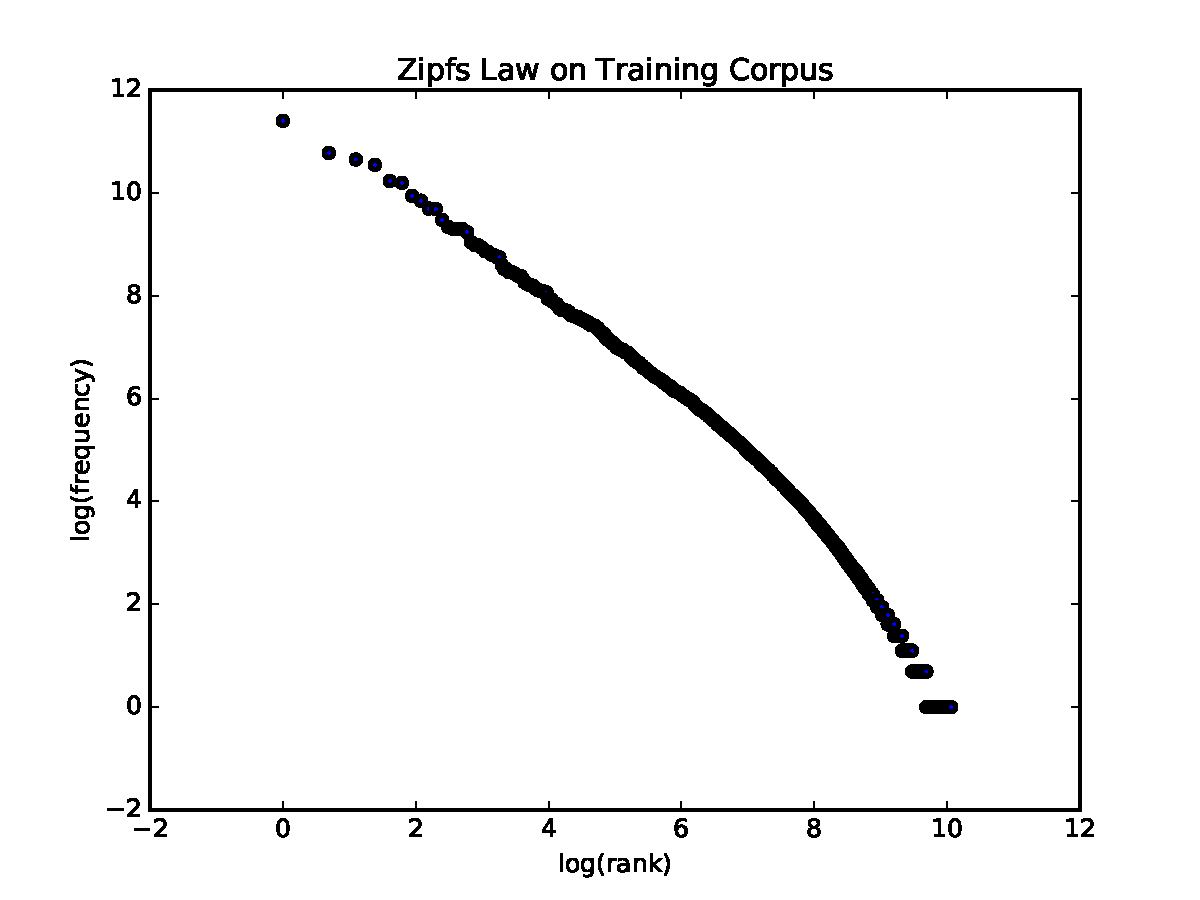
\includegraphics[scale=.5]{zipfslaw.pdf}
\end{center}
\section{Baseline Algorithms}
\noindent
We preformed baseline experiments with Naive Bayes and Support Vector Machine implementations available in Scikit Learn.  We selected the MultinomialNB function for our Naive Bayes classifier because there are three political parties in our dataset, Republican, Democratic, and Independent. The MultinomialNB function includes a smoothing parameter with a default value of 1, but we set this value to 0 as a baseline.  We trained the MultinomialNB classifier on our training data and found that it had an accuracy score of 62.25\% on the test set. We selected the SGDClassifier as our Support Vector Machine implementation because it is flexible and efficient. Specifically it has an option to use multiple cpu's which speeds up the analysis. There are penalty, regularization, class weight and learning hyperparameters which will eventually be tuned using cross validation but all default options were used as a baseline. The SGDClassifier achieved 69.98\% accuracy with no parameter tuning. This is accuracy is notable because [1] Thomas, Pang and Lee report a 70.1\% accuracy predicting a speaker's support or opposition for a policy using this same corpus and similar methods. Political party affiliation is highly correlated with voting behavior, so we are encouraged by this initial result.  We hope that we can achieve higher accuracy by selecting optimal hyper-parameters through cross validation in our final report.

\section{Timeline}
Our next task will be to implement cross validation on each classifier in order to find the optimal hyperparameters. This will enhance our earlier accuracies due to having hyperparameters more suited toward our needs.  Since we have already created a data Pipeline we think this task will be completed shortly. We hope to have this implemented by November 19. The next task on our list will be to create cross validation graphs over the range of hyperparameters that we saw through the process of selecting the hyperparameters. This could help visualize the cross validation selection method as well as provide any information to help solve our problem we're trying to solve. These graphs will be finished by November 26. Next, we will create a draft of our poster for the upcoming poster session as well as any other exhibits that we may need. This will be completed by December 3. After that we will work on the draft of the final paper. This draft will be completed by December 7. Lastly, the finalized paper and poster will be completed by December 10.

\section{Citation}
[1]Thomas, Matt, Bo Pang, and Lillian Lee. ``Get out the Vote: Determining Support or\\\indent Opposition from Congressional Floor-debate Transcripts.'' Proceedings of EMNLP (2006): \indent 327-35. Web. 13 Oct. 2016.\\

\end{document}